\documentclass[12pt, a4paper]{article}
\usepackage{graphicx}
\usepackage[a4paper, total={6in, 8in}]{geometry}
\usepackage{setspace}
\usepackage{parskip}
\usepackage{float}
\usepackage{amsmath}

\begin{document}
\graphicspath{{./images}}

\begin{center}
    \onehalfspacing
    {\Large \textbf{King Fahd University of Petroleum and Minerals} }\\ 
    {\large \textbf{
    College of Computing and Mathematics\\
    Computer Engineering Department 
    } } 
\end{center} 

\begin{figure}[h]
    \centering
    
\includegraphics[width=200px]{images/KFUPM_LOGO.png}
\end{figure}

\begin{center}\onehalfspacing
    \large \textbf{COE 588- Modeling \& Simulation \\of computer and networks Systems }\\
    \normalsize \textbf{Term 232} \\
    \large \textbf{Progress Report}\\
    \textbf{Project}: Simulation and evaluation of M/M/c \\ with an infinite buffer 
\end{center}
\vspace{1em}
\large
\begin{center}
\bgroup
\def\arraystretch{1.3}
\begin{tabular}{|c|c|}
    \hline
    \textbf{Name} & \textbf{KFUPM ID} \\
    \hline
    Hashim Al-Sadah & 201578370\\
    \hline
    Abdulwahab Alghamdi & 201734070\\
    \hline
    Hussain Al-Sinan & 202205120\\
    \hline 
\end{tabular}
\egroup
\end{center}
\vspace{1em}
\begin{center}
    \textbf{Instructor:} Dr. Ashraf S. Hasan Mahmoud.
\end{center}
\normalsize


\onehalfspacing

\section*{Objective}
To simulate the multiple servers queueing system with an infinite buffer, M/M/c, 
and verify that the simulation results match with the theoretical ones. 
The average total time, average waiting time, average number of customers in the system, 
average number of customers in the buffer, and the probability of waiting will 
be simulated as function of the traffic intensity. 
Additionally, the (Probability Density Function) PDF of the total time spent in the system, 
the PDF of the waiting time in the buffer, 
and the (Probability Mass Function) PMF of the number of customers in the system will 
be obtained empirically for low, medium, and high traffic intensity. Finally, we will 
study the effect of increasing the number of servers on the probability of waiting for a fixed
traffic intensity. All the results obtained through simulation will be compared against
the theoretical ones.

\section*{Theoretical Background}
The state diagram for M/M/c is shown in Figure \ref{state_diagram_MMc}. The 
number of servers is denoted by $c$, the arrival rate is $\lambda$, and the 
service rate when the system at some state $s$ is $min(s\mu, c\mu)$.

\begin{figure}[H]
  \centering 
  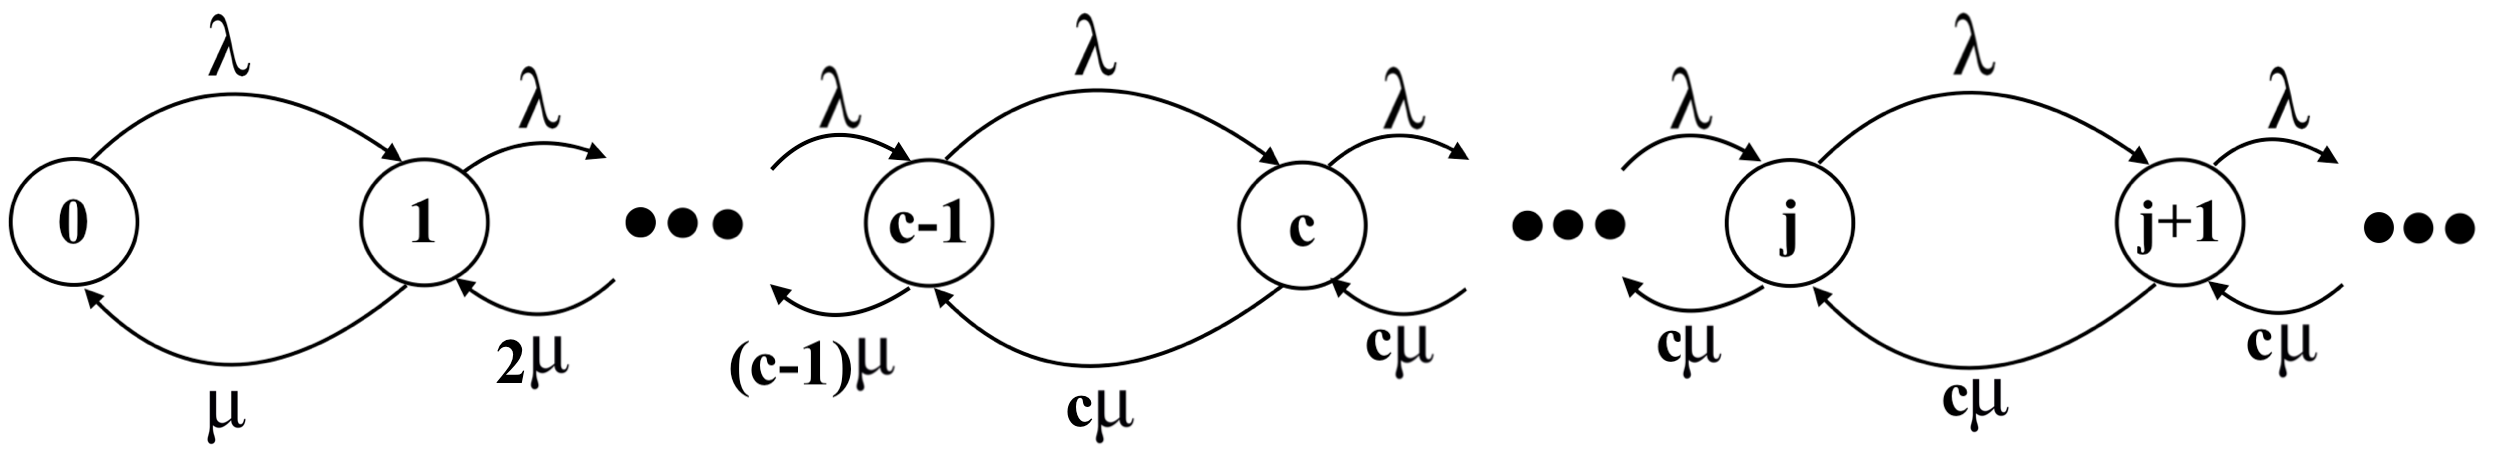
\includegraphics[width=430px]{images/MMc_state_diagram.png}
  \caption{State diagram of M/M/c}
  \label{state_diagram_MMc}
\end{figure}

From the state diagram, one can obtain the global equations and derive 
the equations that describe M/M/c. We will state the equations here without
derivation.

Define $a = \lambda / \mu$. Then the traffic intensity $\rho$ is 
\begin{equation}
  \rho = \frac{a}{c} = \frac{\lambda}{c \mu}
\end{equation}
For all the following equations, we assume that the system is stable. That is 
$\rho < 1$. Then the PMF of $N(t)$ is 
\begin{equation}
  p_0 = \left\{ 
    \left( \sum_{j=0}^{c-1} \frac{a^j}{j!} \right)  
    + \frac{a^c}{c!} \frac{1}{1 - \rho}
    \right\}^{-1}
\end{equation}
\begin{equation}
  p_j = \frac{a^j}{j!} p_0, \quad j = 1, 2, \dots, c
\end{equation}
\begin{equation}
  p_j = \frac{\rho^{j-c}}{c!} a^c p_0, \quad j = c+1, c+2, \dots 
\end{equation}

The probability of having to wait is 
\begin{equation}
  \text{Prob}[\, W > 0 \,] = \text{Prob}[\, N(t) > c \,]
  = \frac{p_c}{1 - \rho}
\end{equation}

The average buffer size is 
\begin{equation}
  E[N_q] = \left( \frac{\rho}{1 - \rho} \right) \text{Prob}
  [\, W > 0 \,]
\end{equation}

The average waiting time is 
\begin{equation}
  E[W] =\frac{E[N_q]}{\lambda}
\end{equation}

The average total time is 
\begin{equation}
  E[T] = E[W] + \frac{1}{\mu}
\end{equation}

The average number of customers in the system 
\begin{equation}
  E[N(t)] = \lambda E[T] = E[N_q] + a  
\end{equation}

The PDF and the CDF of the waiting time, respectively, are 
\begin{equation}
  f_W(t) = c \mu p_c e^{-c \mu \left( 1 - \rho \right)t}, \quad t > 0
\end{equation}
\begin{equation}
  F_W(t) = 1 - \frac{p_c}{1 - \rho} e^{-c \mu \left( 1 - \rho \right)t}, \quad t > 0
\end{equation}

The PDF of the total time is 
\begin{equation}
  f_T(t) = \frac{1}{E[T]} e^{- t/ E[T] }, \quad t \ge 0 
\end{equation}

\section*{Simulation Details}

\section*{Results and Discussion}

\end{document}